\subsection{缓存驻留窗口的推导与逐事件分析}
\subsubsection{先入先出驻留窗口}
缓存时序候选需要判断一次顺序移动究竟试图跨过哪个事件。为此，考察张量 $t$ 在时刻 $f_t$ 成功填入后的这一段驻留期。设其大小为 $b_t\le B_{\mathrm{L2}}$，定义 $A_t(\tau)$ 为 $(f_t,\tau]$ 内在它之后成功新填入队列的对象字节总和。已经在队列中的对象被再次查询或填充时不重复计入；不驻留的超大对象也不计入。这里的“新填入”取自执行事件序列，因此包含不同核心发起请求的全局交错。

\textbf{命题4：}在只按先进先出规则因容量不足淘汰、命中不刷新位置的条件下，张量 $t$ 的首次淘汰发生于第一个使 $b_t+A_t(\tau)>B_{\mathrm{L2}}$ 的新填入事件。在此前的查询时刻，$t$ 仍驻留于缓存。

\textbf{证明：}张量 $t$ 插入时，原队列中的对象均排在它之前。新对象始终排在其后。只要 $t$ 尚未淘汰，排在它之后的对象也不会先被淘汰；故这些对象的实际总大小正是 $A_t(\tau)$。若 $b_t+A_t(\tau)\le B_{\mathrm{L2}}$，即使空间不足，也只需淘汰足够多的旧前缀，仍能容纳 $t$ 及其后的全部对象，无需淘汰 $t$。若首次超过容量，旧前缀即便已全部移除也不足以腾出空间；先进先出规则随后必定淘汰 $t$。由事件次序归纳即得结论。证毕。

因此，若一次消费者读入发射于 $s_t$，要利用这段驻留期，需要该发射在完成填充之后、首次淘汰之前，即落入相应事件序上的区间。设首次淘汰时刻为 $e_t$，对无同刻歧义的事件有
\begin{equation}
 f_t\le s_t<e_t.
 \label{eq:cachewindow}
\end{equation}
若填充、淘汰或查询具有相同周期，还须使用执行器在该周期内的实际事件顺序判断端点；周期相等并不等价于队列状态相同。缓存命中对队列顺序没有影响，所以窗口不能仅由“上一次访问距今多久”描述，而应由填充后进入缓存的字节量及其先后次序描述。这也是缓存时序候选分别尝试调整首次填充、消费者与淘汰者的依据。

式~\eqref{eq:cachewindow} 是固定事件序列的性质。移动子图会改变计算完成、请求发射与带宽共享，进而同时改变 $f_t$、$e_t$ 和 $s_t$。实际方法据原轨迹提出移动方向，再重建整个执行过程；新方案中的驻留窗口随新轨迹重新确定。

\subsubsection{图80的填充、命中与淘汰}
取参数研究中图80的五核固定方案，L2 容量为 $262144$ B，带宽为 $60$ B/周期。图~\ref{fig:q3_trace} 展示原执行中两个张量的事件及开始阶段的读入流水线。为使图中文字易读，将原标识 $1000000001$ 与 $1000000187$ 分别简记为张量甲和张量乙；其大小分别为 $4096$ B 与 $8192$ B。
\begin{figure}[htbp]\centering
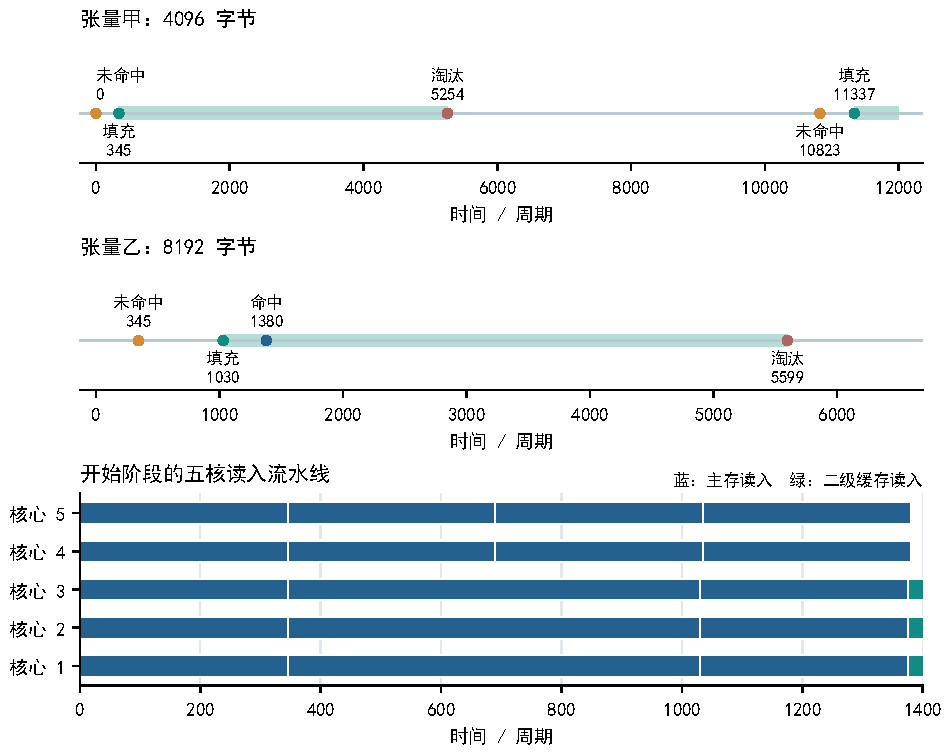
\includegraphics[width=\textwidth]{../求解/问题三/图片/q3_trace.pdf}
\caption{图80的缓存驻留窗口与多核读入轨迹}\label{fig:q3_trace}
\end{figure}

张量甲在周期0的读取未命中，读入于周期345完成后进入缓存。周期5254的一次新填入将它淘汰；当另一核心在周期10823再次读入甲时，访问已落在这段驻留窗口之外，因此再次未命中。甲在周期11337重新填入，于周期15878再次被淘汰；周期21536的下一次读取仍未命中。原图中存在重复消费，但这些消费跨越了有效驻留期，重复本身并未转化为命中。

张量乙在周期345查询时未命中，于周期1030填充；周期1380的查询发生在其驻留期内，因而命中。此命中没有将乙移至队尾，周期5599它仍被后续填入淘汰。两个张量形成直接对照：甲的后续读入晚于淘汰，乙的一次后续读入早于淘汰。顺序候选的目标由此可具体表述为提前某个消费者、推迟造成淘汰的填入者，或提前首次有效填充，而不必将所有重复消费者强制合并到同一子图。

图中最早的五个读请求均在周期0发射、周期345完成，显示共享 DDR 上的并发服务。对甲的 $4096$ B 请求，按每请求独占服务周期向上取整得到 $\lceil4096/60\rceil=69$ 周期；在这五个请求同时在途的区间，共享服务使其完成周期与 $5\times69=345$ 一致。随后各核读入的完成时刻分化，表明请求工作量和在途集合不断变化，不能用固定的五倍因子描述整个执行。

\subsubsection{容量与带宽的非线性作用}
参数格还显示了一个仅看带宽数值容易遗漏的现象：图80在 $262144$ B 容量下，L2 带宽从 $60$ 增至 $250$ 和 $500$ B/周期，周期依次为 $79170$、$80014$ 和 $81744$；图44在 $1048576$ B 容量下，对应周期为 $50723$、$36208$ 和 $44299$。这些值均来自每张图同一完整方案。提高缓存读带宽会提前部分操作，从而改变后续读的发射、完成填充和先进先出队列；在执行状态随之改变的条件下，局部服务变快并不强制整体周期单调下降。

同方案配对中也存在很小的周期反例：图79四核的有 L2 与无 L2 周期分别为 $7614798$ 与 $7614729$，相差69周期，二者额外 COPY 均为 $30445568$ B；该方案字节命中率约为 $0.2804$。相反，图46五核同方案的有 L2 与无 L2 周期分别为 $49119$ 与 $95050$，周期比为 $1.9351$，字节命中率约为 $0.7132$。这些逐例数值与命题4共同说明：缓存评价应追踪关键请求的实际驻留窗口和共享服务，字节命中率适合作为机制指标，总体任务执行时间仍是最终判据。
